\section{Kalibrierung der Brille}

Wie kalibriert man eine Durchsichtbrille in einem Auto?

\subsection{Stereoskopisches 3D}

\subsubsection{Allgemeine Information}
Es existieren mehrere Gründe des menschliches Raumwahrnehmung.
Menschen sehen die Objekte dreidimensional wegen der Linearperspektive, relativer Größe zur anderen Objekte, Verdeckung der Objekten und wegen stereoskopisches Sehen. 
Stereoskopisches Sehen vermittelt durch die beidäugige Betrachtung von Objekten und Gegenständen eine echte, messbare Tiefenwahrnehmung und räumliche Wirkung des Außenraums. 
Das passiert mit der Hilfe beider unseren Augen.
Jede Auge bekommt ein eigenes Bild und sendet das ins Gehirn. 
Dort werden diese beide Bilder zu eine einzige zusammengefasst.
Genauere Beschreibung ist im Abb. \ref{fig:3D} zu finden.

\begin{figure}[h]
   \centering
   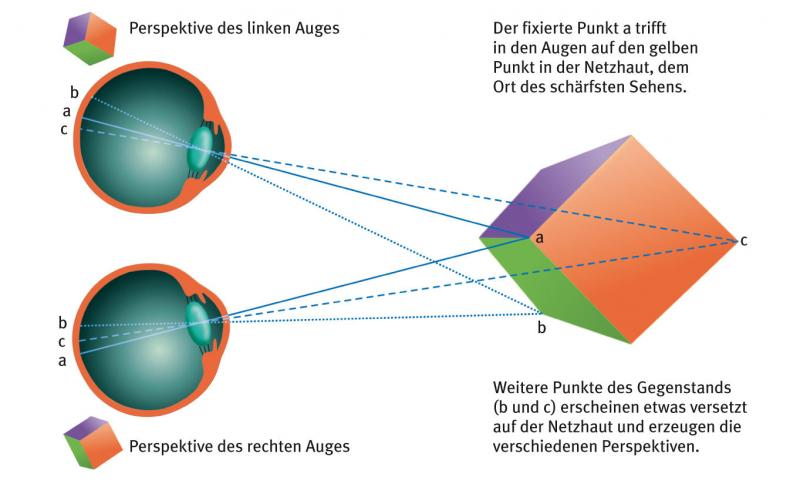
\includegraphics[width=0.45\textwidth]{3D-bild}
   \caption{steteoskopisches Sehen}
   \label{fig:3D}
\end{figure}

Die Bilder des linken und rechten Auges sich an manchen Stellen unterscheiden und menschliches Gehirn kann aus dieser Unterschiede die Positionen, Formen und Großen der Objekte extrahieren.

Damit ein Bild dreidimensional aussieht, ist meistens genug mit ungefähren Werten zu arbeiten.
Man nimmt zwei unterschiedliche Bilder, die anhand der mittlere Werte ausgerechnet werden, und zeigt jeder Auge eine davon. 
Damit bekommt man ein 3D-Bild. 
Für manche Anwendungen (wie 3D-Filme, oder sterioskopische Bilder) ist schon genug,  dass ein Bild als 3D interpretiert wird. 
Für uns aber nicht, da mit so eine Realisation unterschiedliche Menschen sehen dasselbe Bild unterschiedlich.
Alle Menschen werden diese Bilder als 3D interpretieren, aber die Position und Größe der gesehenen Objekte kann sich stark unterscheiden.
Für die Anwendungen, wie Testen des autonomes Fahrens des Fahrzeugs, sind aber diese Werte entscheidend.
Es ist sehr wichtig, ob ein anderes Fahrzeug schon getroffen ist, oder nicht.
Um die benötigte Genauigkeit zu realisieren, sind gemittelte Werte nicht genug.
Eine individuelle Kalibrierung der Brille soll diese Genauigkeit ermöglichen.

\subsubsection{Geometrische Beschreibung der Kalibrierung}
Dieses Kapitel beschreibt wofür die Kalibrierung durchgeführt wird und welche Daten dafür benötigt werden.
Die gegebene Daten sind im Abb. \ref{fig:geom} dargestellt. 

\begin{figure}[h]
   \centering
   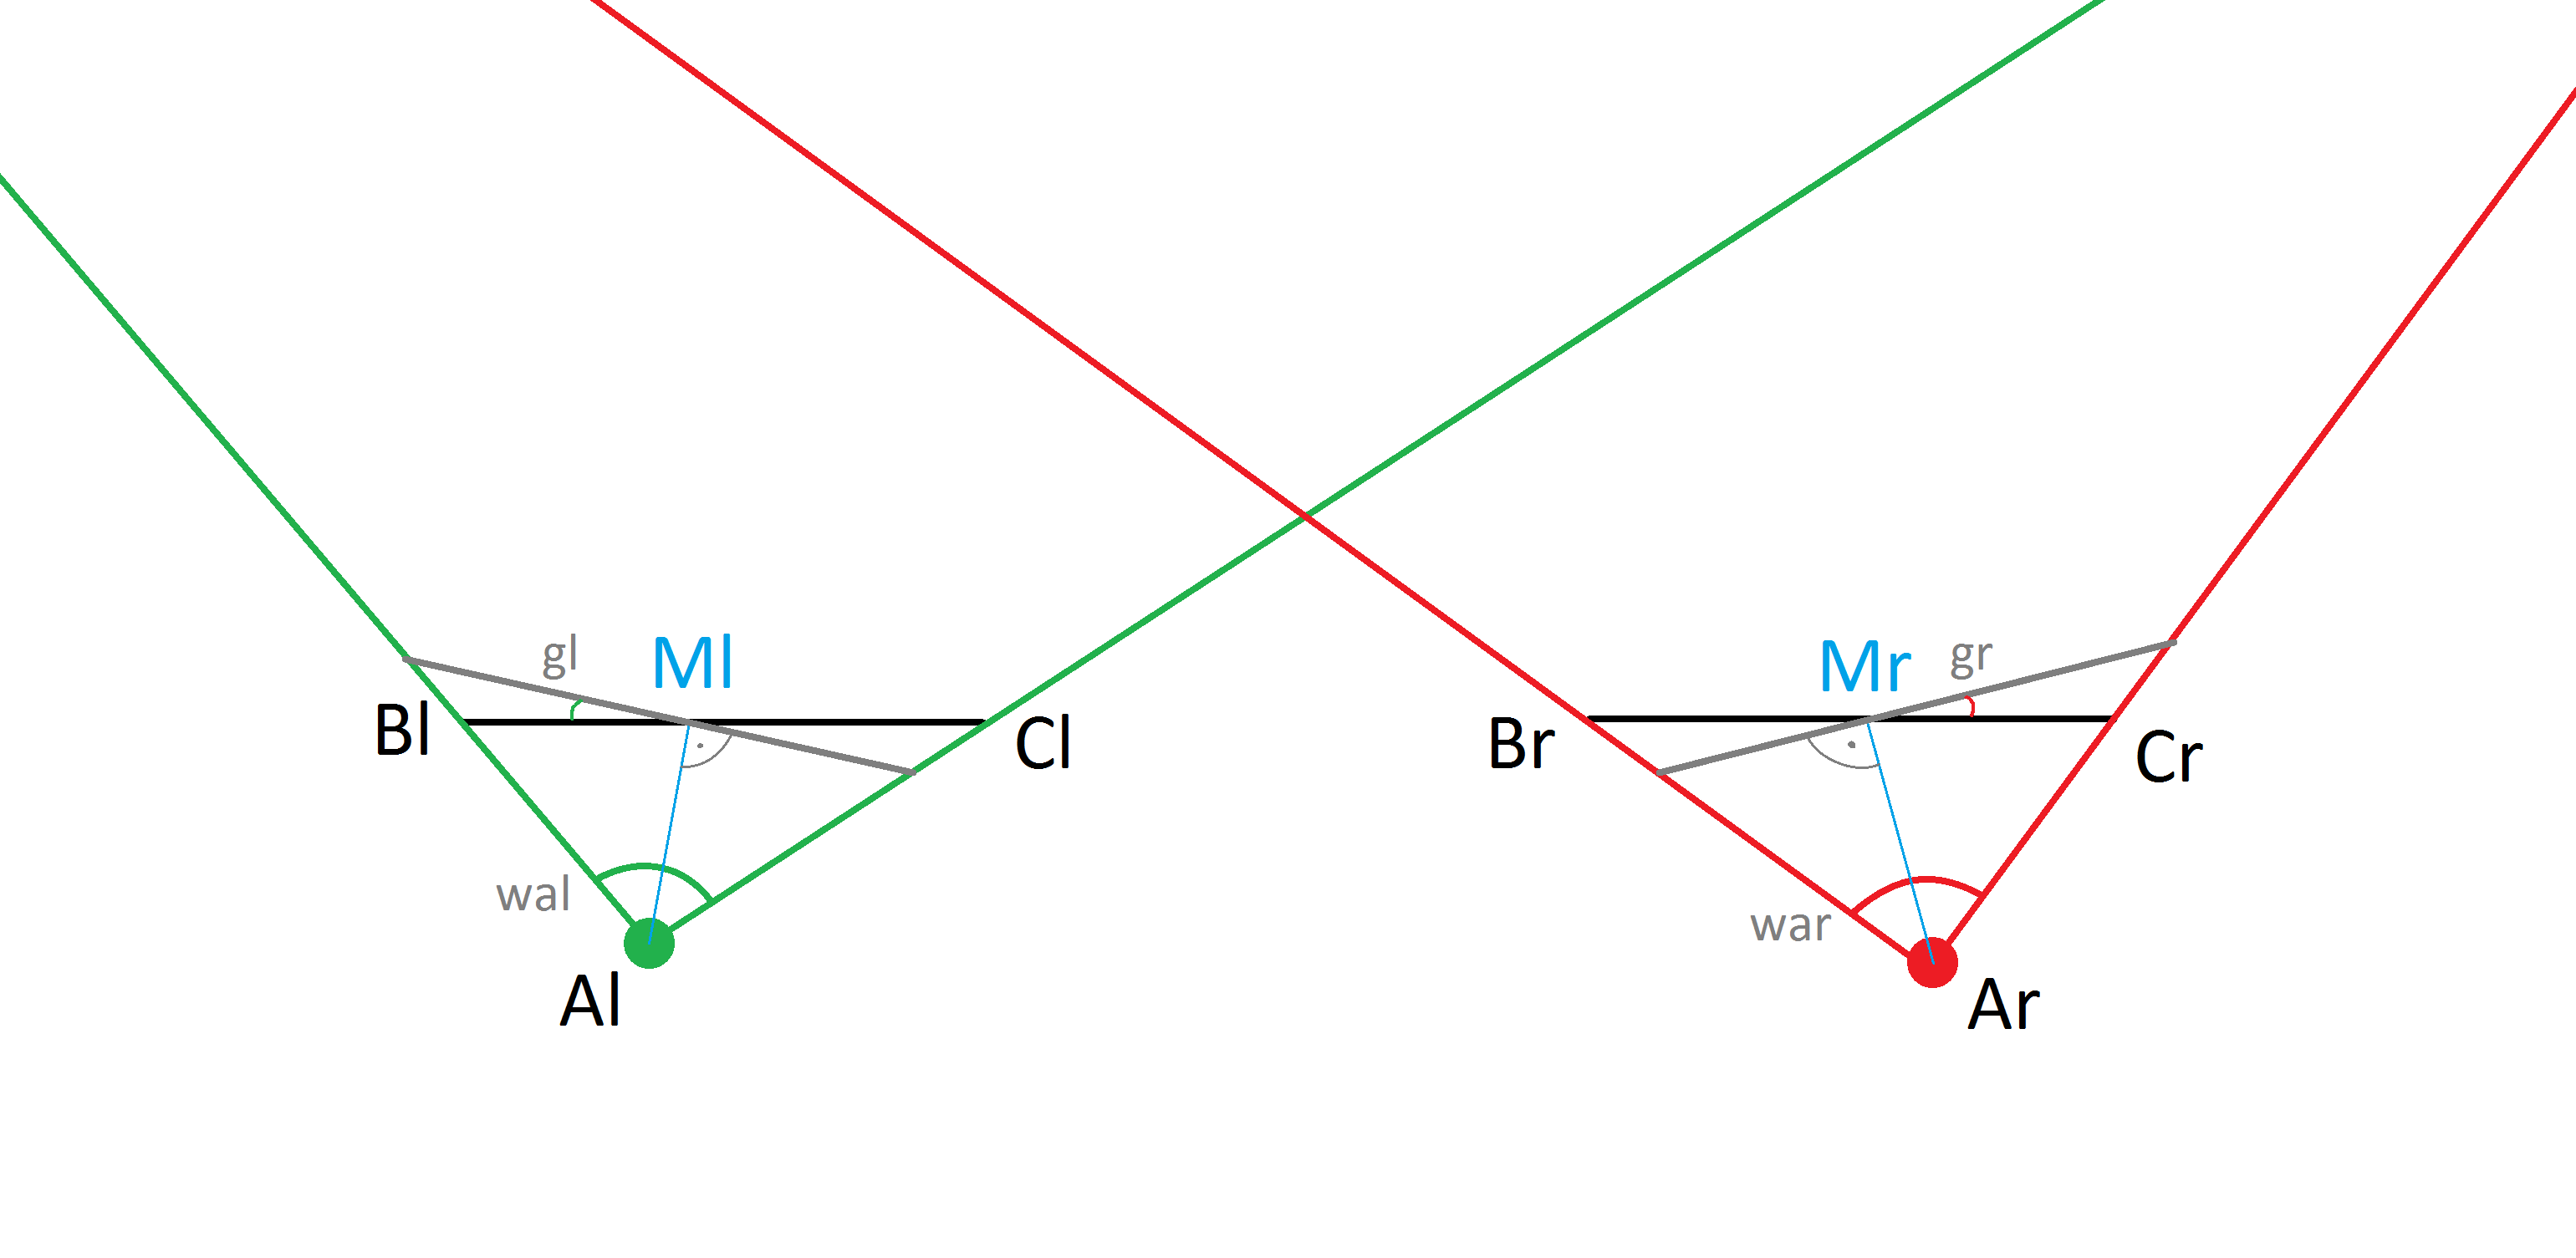
\includegraphics[width=0.45\textwidth]{kalibr-geometrie}
   \caption{Geometrische Beschreibung der Kalibrierung}
   \label{fig:geom}
\end{figure}

Punkte Bl, Cl bzw. Br, Cr sind die Endpunkte des linkes bzw. rechtes Bildschirms der Brille.
Die Punkte Al (grün) bzw. Ar (rot) beschreiben die Positionen der Augen.
wal bzw. war sind die Sehwinkel des Benutzers durch welche die Bildschirme und dort dargestellte Objekte gesehen werden. 
Blaue Linien ml und mr sind Winkelhalbierenden.

Für die Anzeige der Bilder auf der Brillenbildschirme, werden Augen als Kameras interpretiert und damit werden benötigte Bilder erstellt.
Dementsprechend sind die Winkeln wal und war die Öffnungswinkel dieser Kameras.
Wie auf dieser Abb. ref{fig:geom} gut zu sehen ist, müssen die Augepositionen nicht unbedingt in der mitte des Bildschirms liegen.
In meisten Anwendungen, die Kameras simulieren, ist aber vorausgesetzt, dass die Kameras in der Mitte sind.
Das ist das selbe, wie Winkelhalbierende der Öffnungswinkel senkrecht zur Bildschirm ist.
Wir nehmen an, dass dafür benötigte Drehwinkel gl bzw. gr spielt keine entscheidende Rolle in der Bildanzeige.
Mit dieser Annahme rechnen wir die Winkeln gl und gr aus  um die Virtuelle Bildschirme theoretisch zu drehen.
Das wird benötigt um passende Daten für die Benutzung anderer Anwendungen zu bekommen.



